\documentclass[
	classe=$1^{ere}STI2D$,
]{exercice}

\usepackage{xargs}

\renewcommand{\arraystretch}{1.3}
\newcommandx{\Graphe}[5][4=-4,5=4]{
	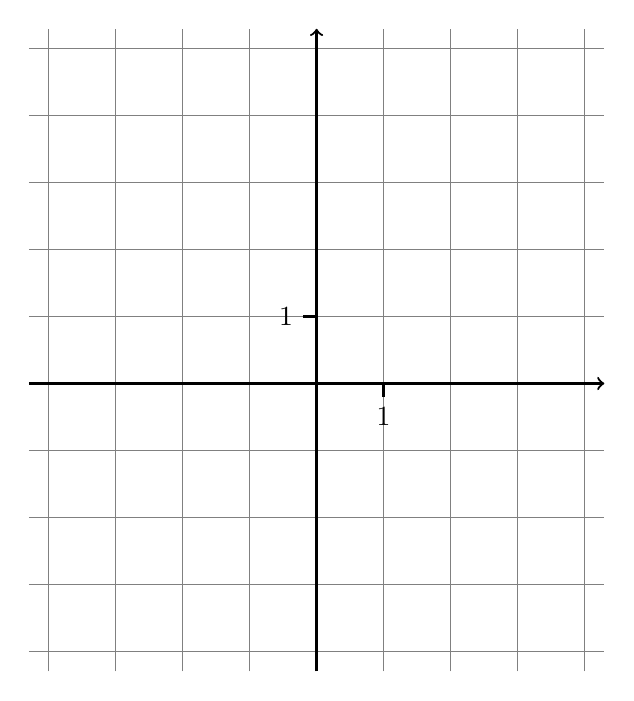
\begin{tikzpicture}[scale=0.85]
		\draw[thin,gray] (-4.3,-4.3) grid (4.3,5.3);
		\draw[thick,->] (-4.3,0) -- (4.3,0);
		\draw[thick,->] (0,-4.3) -- (0,5.3);
		\draw[thick] (1,0) -- ++(0,-0.2) node[below] {$1$};
		\draw[thick] (0,1) -- ++(-0.2,0) node[left] {$1$};

		\ifdefined\makeCorrection
			\draw[variable=\x,domain=#4:#5,red] plot({\x},{#1*\x*\x + #2*\x + #3});
		\fi
	\end{tikzpicture}
}

\title{Courbes de fonctions de degré 2}

\begin{document}

\maketitle

Pour chaque fonction, donner les coefficients $a$, $b$ et $c$, et s'en servir pour faire un tracé rapide de la courbe.

\begin{multicols}{2}
	\begin{enumerate}
		\item $f(x) = -\dfrac{1}{4}x² + \dfrac{1}{2}x + 2$ \hspace{2em} \begin{tabular}{l}
			      $a = \correctionOr{-\dfrac{1}{4}}{.....}$ \\
			      $b = \correctionOr{\dfrac{1}{2}}{.....}$  \\
			      $c = \correctionOr{2}{.....}$
		      \end{tabular}

		      Donc $a\ \correctionDots{<}\ 0$, et $-\dfrac{b}{2a} = \correctionDots{1}$.

		      \begin{center}
			      \Graphe{-1/4}{1/2}{2}
		      \end{center}
		\item $g(x) = \dfrac{1}{6}x² + \dfrac{1}{3}x - 1$ \hspace{2em} \begin{tabular}{l}
			      $a = \correctionOr{\dfrac{1}{6}}{.....}$ \\
			      $b = \correctionOr{\dfrac{1}{3}}{.....}$  \\
			      $c = \correctionOr{-1}{.....}$
		      \end{tabular}

		      Donc $a\ \correctionDots{>}\ 0$, et $-\dfrac{b}{2a} = \correctionDots{-1}$.

		      \begin{center}
			      \Graphe{1/6}{1/3}{-1}
		      \end{center}
		\item $h(x) = x² - 4$ \hspace{2em} \begin{tabular}{l}
			      $a = \correctionOr{1}{.....}$ \\
			      $b = \correctionOr{0}{.....}$  \\
			      $c = \correctionOr{-4}{.....}$
		      \end{tabular}

		      Donc $a\ \correctionDots{>}\ 0$, et $-\dfrac{b}{2a} = \correctionDots{0}$.

		      \begin{center}
			      \Graphe{1}{0}{-4}[-3][3]
		      \end{center}
		\item $i(x) = -\dfrac{1}{4}(x + 4)(x - 2)$ \hspace{2em} \begin{tabular}{l}
			      $a = \correctionOr{-\dfrac{1}{4}}{.....}$ \\
			      $b = \correctionOr{-\dfrac{1}{2}}{.....}$  \\
			      $c = \correctionOr{2}{.....}$
		      \end{tabular}

		      Donc $a\ \correctionDots{<}\ 0$, et $-\dfrac{b}{2a} = \correctionDots{-1}$.

		      \begin{center}
			      \Graphe{-1/4}{-1/2}{2}
		      \end{center}
	\end{enumerate}
\end{multicols}

\end{document}